\chapter{Dataset}
In questo capitolo viene analizzato il dataset. Viene quindi spiegato da dove è stato preso il dataset, descritte le covariate e viene effettuata un'analisi esplorativa.

\section{Acquisizione del dataset}
Il dataset completo contenente informazioni sui singoli e riguardo le varie certificazioni non è disponibile da una sola sorgente. Pertanto abbiamo ottenuto le informazioni necessarie da diversi sorgenti per poi integrare i dati.

\subsection{Dataset spotify - Kaggle}
Per quanto riguarda i brani con le relative informazioni e caratteristiche del brano, Spotify mette a disposizone un'API da cui si possono ottenere questi dati.

Con questa tecnica sono stati ottenuti i dati relativi ai brani, un utente ha quindi caricato il dataset sul sito \href{https://www.kaggle.com/}{kaggle.com}. Il dataset è disponibile su kaggle all'url indicato. \footnote{\textbf{Dataset Spotify}: \href
	{https://www.kaggle.com/yamaerenay/spotify-dataset-19212020-160k-tracks}
	{https://www.kaggle.com/yamaerenay/spotify-dataset-19212020-160k-tracks}.}.

Il dataset contenente queste informazioni è il file: \verb|data/raw/to_integrate/data.csv|
\subsection{Premi canzoni - Wikipedia}
Le informazioni riguardo i premi delle canzoni, ovvero le varie certificazioni vinte, sono disponibili su \href{https://it.wikipedia.org//}{wikipedia.org}. 

Nello specifico siamo interessati a:
\begin{itemize}
	\item Singoli certificati oro
	\item Singoli certificati platino
	\begin{enumerate}
		\item Singoli certificati 1 volta platino
		\item Singoli certificati 2 volte platino
		\item ...
		\item Singoli certificati N volte platino
	\end{enumerate}
\end{itemize}

Inoltre le varie certificazioni dei singoli vengono considerati in base al paese. I paesi da noi presi in considerazione sono:
\begin{enumerate}
	\item Italia
	\item Australia
	\item Stati Uniti d'America
	\item Regno Unito
	\item Canda
	\item Danimarca
\end{enumerate}
Si noti come una certificazione può essere consegnata in diversi paesi alla stessa canzone.

\subsubsection{Certificazioni disco d'oro}
Per quanto riguarda i dischi d'oro, facciamo riferimento a questa pagina su wikipedia \footnote{\textbf{Disco d'oro per stato}:\\
	\href
	{https://it.wikipedia.org/wiki/Categoria:Singoli_certificati_oro_per_stato}
	{https://it.wikipedia.org/wiki/Categoria:Singoli\_certificati\_oro\_per\_stato}.}.
Fissato quindi uno stato (ad esempio l'Italia) è possibile visualizzare la pagina contenente la lista dei singoli che hanno vinto quel particolare premio. La lista è un elenco di url che puntano alla pagina wikipedia della canzone, un esempio a questo url\footnote{\textbf{Singoli certificati disco d'oro in Italia}:\\
	\href
	{https://it.wikipedia.org/wiki/Categoria:Singoli\_certificati\_disco\_d\%27oro_in_Italia}
	{https://it.wikipedia.org/wiki/Categoria:Singoli\_certificati\_disco\_d\%27oro\_in\_Italia}.}.

\subsubsection{Certificazioni disco di platino}
Ragionamento analogo viene fatto per i dischi di platino, con l'unica differenza che la pagina è questa\footnote{\textbf{Singoli certificati disco di platino per stato}:\\
	\href
	{https://it.wikipedia.org/wiki/Categoria:Singoli_certificati_platino_per_stato}
	{https://it.wikipedia.org/wiki/Categoria:Singoli\_certificati\_platino\_per\_stato}.}, inoltre
dal momento che i singoli posso vincere più volte un disco di platino, si considerano non solo i singoli che hanno vinto una volta il discho di platino ma anche quelli che l'hanno vinto N volte.

\subsubsection{Scraping}
Ottenuti quindi i puntatori alle canzoni certificate, è possibile accedere alla pagina wikipedia del singolo, la quale contiene una tabella riassuntiva della canzone. Un esempio di tabella viene mostrato nella Figura \ref{fig:wiki_table}.
\begin{figure}[H]
	\centering
	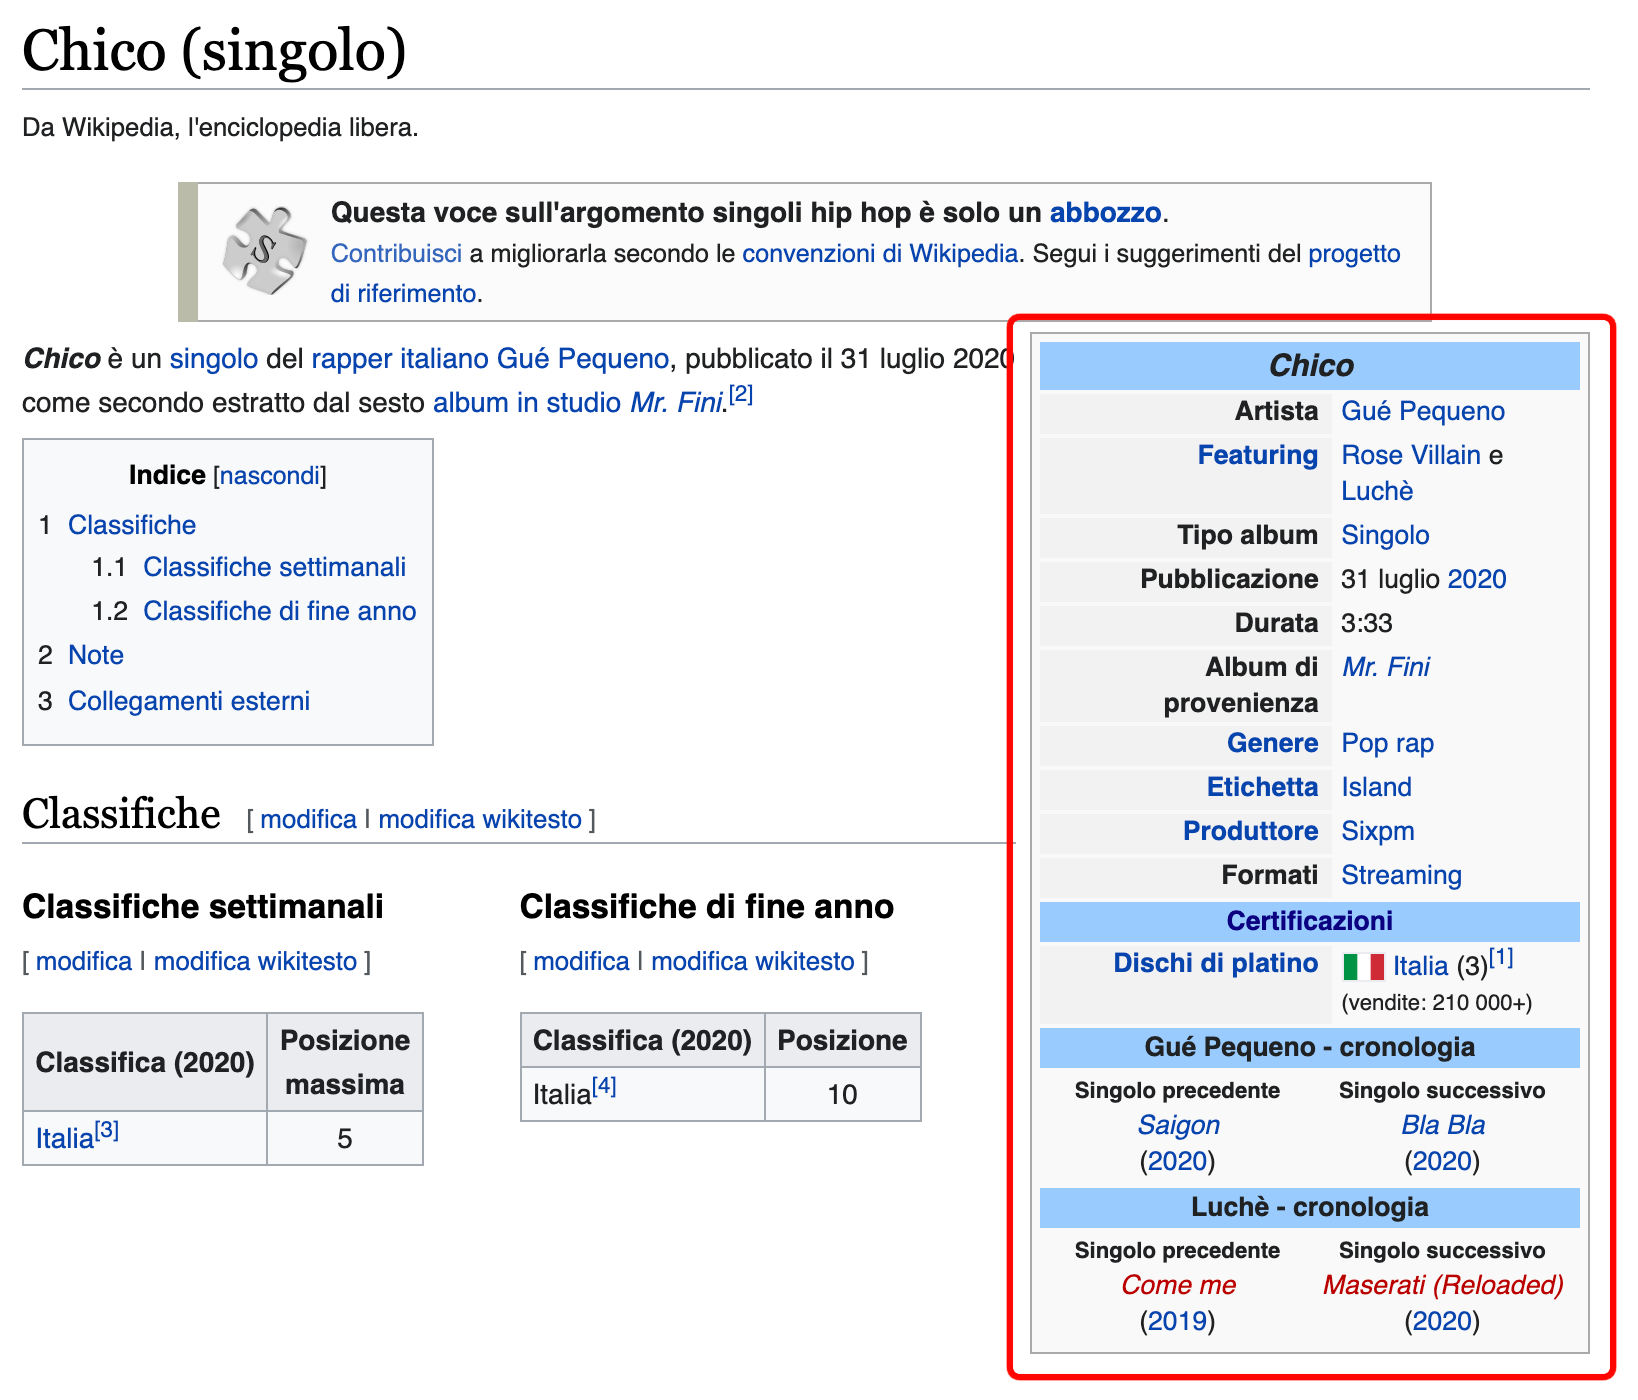
\includegraphics[width=12cm]{assets/wikipedia-table.png}
	\caption{Esempio di tabella per un singolo musicale su wikipedia}
	\label{fig:wiki_table}
\end{figure}

Viene quindi creato uno script per effettuare scraping delle tabelle, il codice è nella directory\\ \verb|scraping/wikipedia_songs_scraper.py|.

Successivamente si integrano le informazioni dei diversi stati, e tipi di certificazione vinti. Il risultato di questa operazione è il file \verb|data/raw/to_integrate/awards_cleaned.csv|.

\section{Descrizione del dataset}
In questa sezione vengono elencate e descritte le features del dataset.
\subsection{Spotify}
\label{sec:descrizione_spotify}
Di seguito viene descritto il dataset proveniente da kaggle, ovvero quello contenente le informazioni dei brani.

\begin{center}
	
	\resizebox{\textwidth}{!}{
		\begin{tabular}[H]{ |l|l|l| }
			\hline
	
			\multicolumn{1}{ |c }{\textbf{ATTRIBUTO}} &
			\multicolumn{1}{ c }{\textbf{DESCRIZIONE}} &
			\multicolumn{1}{ c| }{ \textbf{TIPO}} \\
			
			\hline
			\hline
			
			id & 
			Identificativo della canzone (generato da spotify) &
			Intero\\
			
			name & 
			Titolo della canzone &
			Stringa\\
			
			artists & 
			Lista degli artisti che compaiono nel brano &
			Stringa\\
			
			year & 
			Anno del brano &
			Intero\\
			
			duration\_ms & 
			Durata della traccia in millisecondi &
			Intero\\
			
			acousticness & 
			Metrica riguardante quanto un brano risulta "acustico" &
			Float [0, 1]\\
			
			danceability & 
			Metrica riguardante quanto una traccia è ballabile &
			Float [0, 1]\\
			
			energy & 
			Energia del brano &
			Float [0, 1]\\
			
			explicit & 
			Indica se la traccia è esplicita oppure no (linguaggio volgare) &
			Binario\\
			
			instrumentalness & 
			Contenuto relativo di strumenti musicali nella traccia&
			Float [0, 1]\\
			
			valence & 
			Metrica riguardante la "positività" della traccia &
			Intero\\
			
			key & 
			Chiave musicale utilizzata &
			Intero [0, 11]\\
			
			liveness & 
			Durata relativa della traccia suonata in una performance dal vivo &
			Float [0, 1]\\
			
			loudness & 
			Rumorosità della traccia in decibel (dB) &
			Float [-60, 0]\\
			
			mode & 
			Indica se la traccia parte con una progressione armonica &
			Booleano\\
			
			release\_date & 
			Anno di rilascio del brano&
			Intero\\
			
			speechiness & 
			Contenuto relativo di voce umana nella traccia &
			Float [0, 1]\\
			
			tempo & 
			BPM della traccia &
			Float\\
			
			popularity & 
			Popolarità della traccia &
			Float [0, 100]\\
			\hline
			
		\end{tabular}
	}
\end{center}



\subsection{Premi}
Si noti come la distinzione tra tipo di premio vinto e lo stato in cui è stata ottenuta la certificazione per uno specifico brano, viene fatta solo a scopo dello scraping, in quanto i brani sono così rappresentati sul sito di wikipedia. Tuttavia da questo punto in poi non verrà più tenuto conto di questa informazione, infatti un singolo verrà considerato come\textbf{ vincitore di un premio} (e quindi di successo) oppure come \textbf{non vincitore di un premio} (non di successo). 

Il risultato dello scraping della tabella di wikipedia è il seguente:


\begin{center}
	
	\resizebox{\textwidth}{!}{
		\begin{tabular}[H]{ |l|l|l| }
			\hline
			
			\multicolumn{1}{ |c }{\textbf{ATTRIBUTO}} &
			\multicolumn{1}{ c }{\textbf{DESCRIZIONE}} &
			\multicolumn{1}{ c| }{ \textbf{TIPO}} \\
			
			\hline
			\hline
			
			title & 
			Titolo della canzone &
			Stringa\\
			
			artists & 
			Artisti presenti nela traccia &
			Stringa\\
			
			date & 
			Data di rilascio della traccia &
			Data\\
			
			genre & 
			Genere musicale del brano&
			Stringa\\
			
			award & 
			Premio vinto dal singolo&
			Stringa \{Oro, 1\_platino, 2\_platino, ...\}\\
			
			nation & 
			Paese in cui è stato vinto il premio&
			Stringa (Sigla del paese)\\
			\hline
			
		\end{tabular}
	}
\end{center}


\section{Normalizzazione}
OpenRefine con regex per le date

\section{Data integration}
Possiamo etichettare i brani come di successo oppure non di successo.
\subsection{Modellazione struttura documentale}
\subsection{Record linkage con MongoDB}
Una roba veloce giusto per spiegare

\begin{enumerate}
	\item Import dati mongodb
	\item Creazione indici
	\item Preprocessing lowercase
	\item Unfold campo artista
	\item Record linkage -> Join basandosi su titolo e artisti
	\item Lista artisti come stringa
	\item Dump del database in un file .csv come risultato del dataset per i modelli
\end{enumerate}



\section{Analisi esplorativa}

\subsection{Distribuzione dei valori}
\subsubsection{Variabili continue}
\subsubsection{Variabili categoriche}

\subsection{Artisti nelle canzoni}
\subsubsection{Frequenza artisti}
\subsubsection{Wordcloud}


\subsection{Correlazione features}

\subsection{Principal component analysis}
Prima di PCA normalizzazione del dataset

NB: Non facciamo il plot delle prime due componenti principali in quanto varianza spiegata dalle prime due componenti molto bassa

\subsection{Creazione dataset bilanciato}
\subsubsection{Undersampling}


\section{Scelta delle features}
\subsection{Normalizzazione e standardizzazione}
Conversione in lowecase
Converto in variabili numeriche e factor + label corretta
\subsection{Dataset proiettato componenti principali}
\subsection{Variabili categoriche}
\subsubsection{Key -> Trasformazione a intero}
\subsection{Artisti in una canzone - BOW}
\subsubsection{Threshold freqeunza}
Viene usato un threshold a 2 per non avere delle canzoni con artisti completamente sconosciuti. Assumiamo quindi di fare previsioni su canzoni cantante da artisti un minimo conosciuti.

Questa assunzione non è molto restrittiva, ci immaginiamo infatti che per vincere un premio una canzone deve essere cantata da artisti non completamente sconosciuti

Inoltre a causa dell'undersampling è possibile avere diverse canzoni cantate da artisti "sconosciuti" e non avendo scelto una particolare strategia per l'undersampling adottiamo a questo punto l'utilizzo di un threshold

\subsection{Popularity}
Chiaramente questa feature viene scartata per non creare modelli biased (Non si conosce questa feature quando una canzone esce)
